\documentclass{article}
\usepackage{geometry}
\geometry{a4paper}
\usepackage{amsmath}
\usepackage{empheq}
\usepackage{mhchem} % Package for chemical equation typesetting
\usepackage{siunitx} % Provides the \SI{}{} command for typesetting SI units
\usepackage{parskip}
\usepackage{graphicx} % Required for the inclusion of images
\usepackage{amssymb}
\usepackage{placeins}
\usepackage{cancel}
\usepackage{fullpage}
%\usepackage{subfig}
\usepackage{enumitem}
\usepackage{listings}
%\usepackage{mcode}
\usepackage{wrapfig}
%\renewcommand{\labelenumii}{\alph{enumi}.}
%Alph for uppcer case, \arabic for 1, 2, 3
%\roman for i, ii, iii \alph{enumi})
% Make numbering in the enumerate environment by letter rather than number (e.g. section 6)
\usepackage{booktabs, multicol, multirow}
%\usepackage[ ]{mcode} 

\setlength\parindent{0pt} % Removes all indentation from paragraphs

\renewcommand{\labelenumi}{\alph{enumi}.} % Make numbering in the enumerate environment by letter rather than number (e.g. section 6)

%\usepackage{times} % Uncomment to use the Times New Roman font

\include{paulsmacros}
%\braces , \parens \brackets \mC (matrix C) \vv (vector v) \h hats for somethings ie \hvy or \hmA \sA (subscript upper case)
\usepackage{caption}
\usepackage{subcaption}

%----------------------------------------------------------------------------------------
%	DOCUMENT INFORMATION
%----------------------------------------------------------------------------------------
%$\frac{-1}{\sqrt{a}}$
%\title{Newberry/Felix  \hfill \today}
%\date{}
\begin{document}
%\maketitle 
%\LARGE
\textsc{\Large Fluid Solver Validation \hfill \today}\\[0.5cm] % Name of your university/college
\textsc{\large Felix Newberry}\\

This report describes the validation of a Fenics fluid solver. The code in question can be found in the Github repository under \verb|/2_Cylinder_benchmark/cylinder_navier-stokes.py|. 

\section{Problem Setup} 

The fluid problem is solved with an Incremental Pressure Correction Scheme (IPCS). The fluid solver is validated with a 2D benchmark channel flow past a circular cylinder \cite{schafer1996benchmark}. 

\subsection{Geometry}
The geometry of the problem is depicted in Figure \ref{fig:geom}. 

\FloatBarrier
\begin{figure}[h]
\centering
	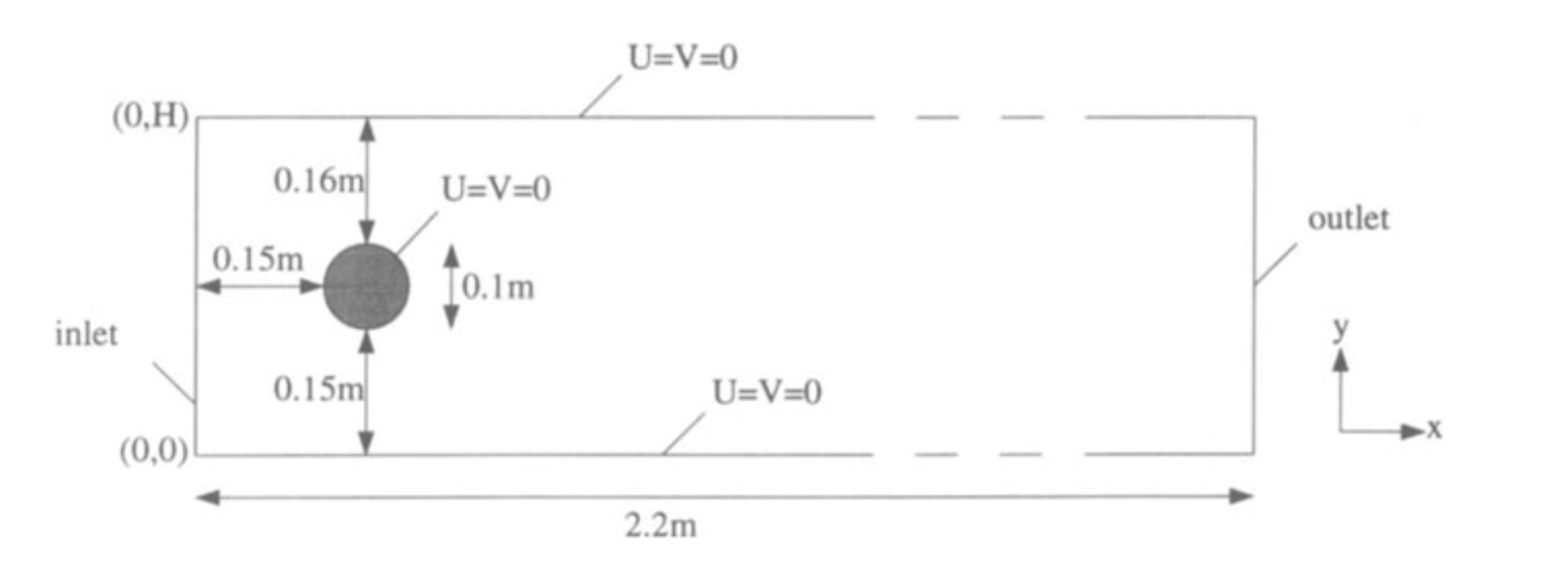
\includegraphics[width=\textwidth]{geometry}
	\caption{Fluid test case geometry \cite{schafer1996benchmark}}
	\label{fig:geom}
\end{figure}
\FloatBarrier

A circular cylinder of diameter $D = 0.1 m$ is placed slightly off center in a channel of height $H = 0.41 m$.  is the channel height and  the 

\subsection{Boundary Conditions}
The channel walls are no-slip condition while the outlet pressure is set to 0. The inflow is a parabolic velocity profile in the x direction defined as 

\begin{equation}
U(0, y) = \frac{4 U_m y (H - y)}{H^2} , V = 0
\end{equation}

Where $U_m = 0.3$ is the maximum velocity of the inlet and the mean velocity is defined as $\bar{U}$ 

\subsection{Fluid Properties}
The fluid considered is incompressible and Newtonian. The kinematic viscosity was defined as $\nu = 0.001 m^2s^{-1}$ and the density as $ \rho = 1.0 kg m^{-3}$. 

\subsection{Validation Metrics}
The metrics for validation are the drag and lift coefficents $c_D$ and $c_L$ the change in pressure between the front and back of the cylinder. The drag and lift forces were calculated as 

\begin{equation}
F_D = \int ( \rho \nu \frac{\partial v_t}{\partial n}  n_y - P n_x ) dS
\end{equation}

\begin{equation}
F_L = - \int ( \rho \nu \frac{\partial v_t}{\partial n}  n_x - P n_y ) dS
\end{equation}

Where $S$ denotes the cylinder, $n$ is the normal vector on $S$ with x and y components $n_x$ and $n_y$. $v_t$ is the tangential velocity on $S$ with tangent vector $t = (n_y - n_x)$ and $P$ is the pressure. 

The drag and lift coefficients are calculated

\begin{equation}
c_D = \frac{2 F_D}{\rho \bar{U}^2 D}
\end{equation}

\begin{equation}
c_L = \frac{2 F_L}{\rho \bar{U}^2 D}
\end{equation}

The change in pressure $\Delta P$ is calculated as $\Delta P(t) = P(0.15, 0.2, t) -  P(0.25, 0.2, t)$. 

\subsection{Mesh}

The Mesh used in this analysis was created in Fenics. A mesh parameter $N$ defined both the number of facets on the cylinder and was the input resolution to the Fenics command \verb|/generate_mesh(geometry,N)|. In addition, a refinement box was applied with vertices $(0.1, 0.1)$, and $(0.8, 0.3)$ in order to better capture the dynamics close to and in the wake of the cylinder. The respective meshes for $N = 32$ and $N = 256$ are displayed in Figure \ref{fig:mesh}. 

\FloatBarrier
\begin{figure}[h]
\centering
	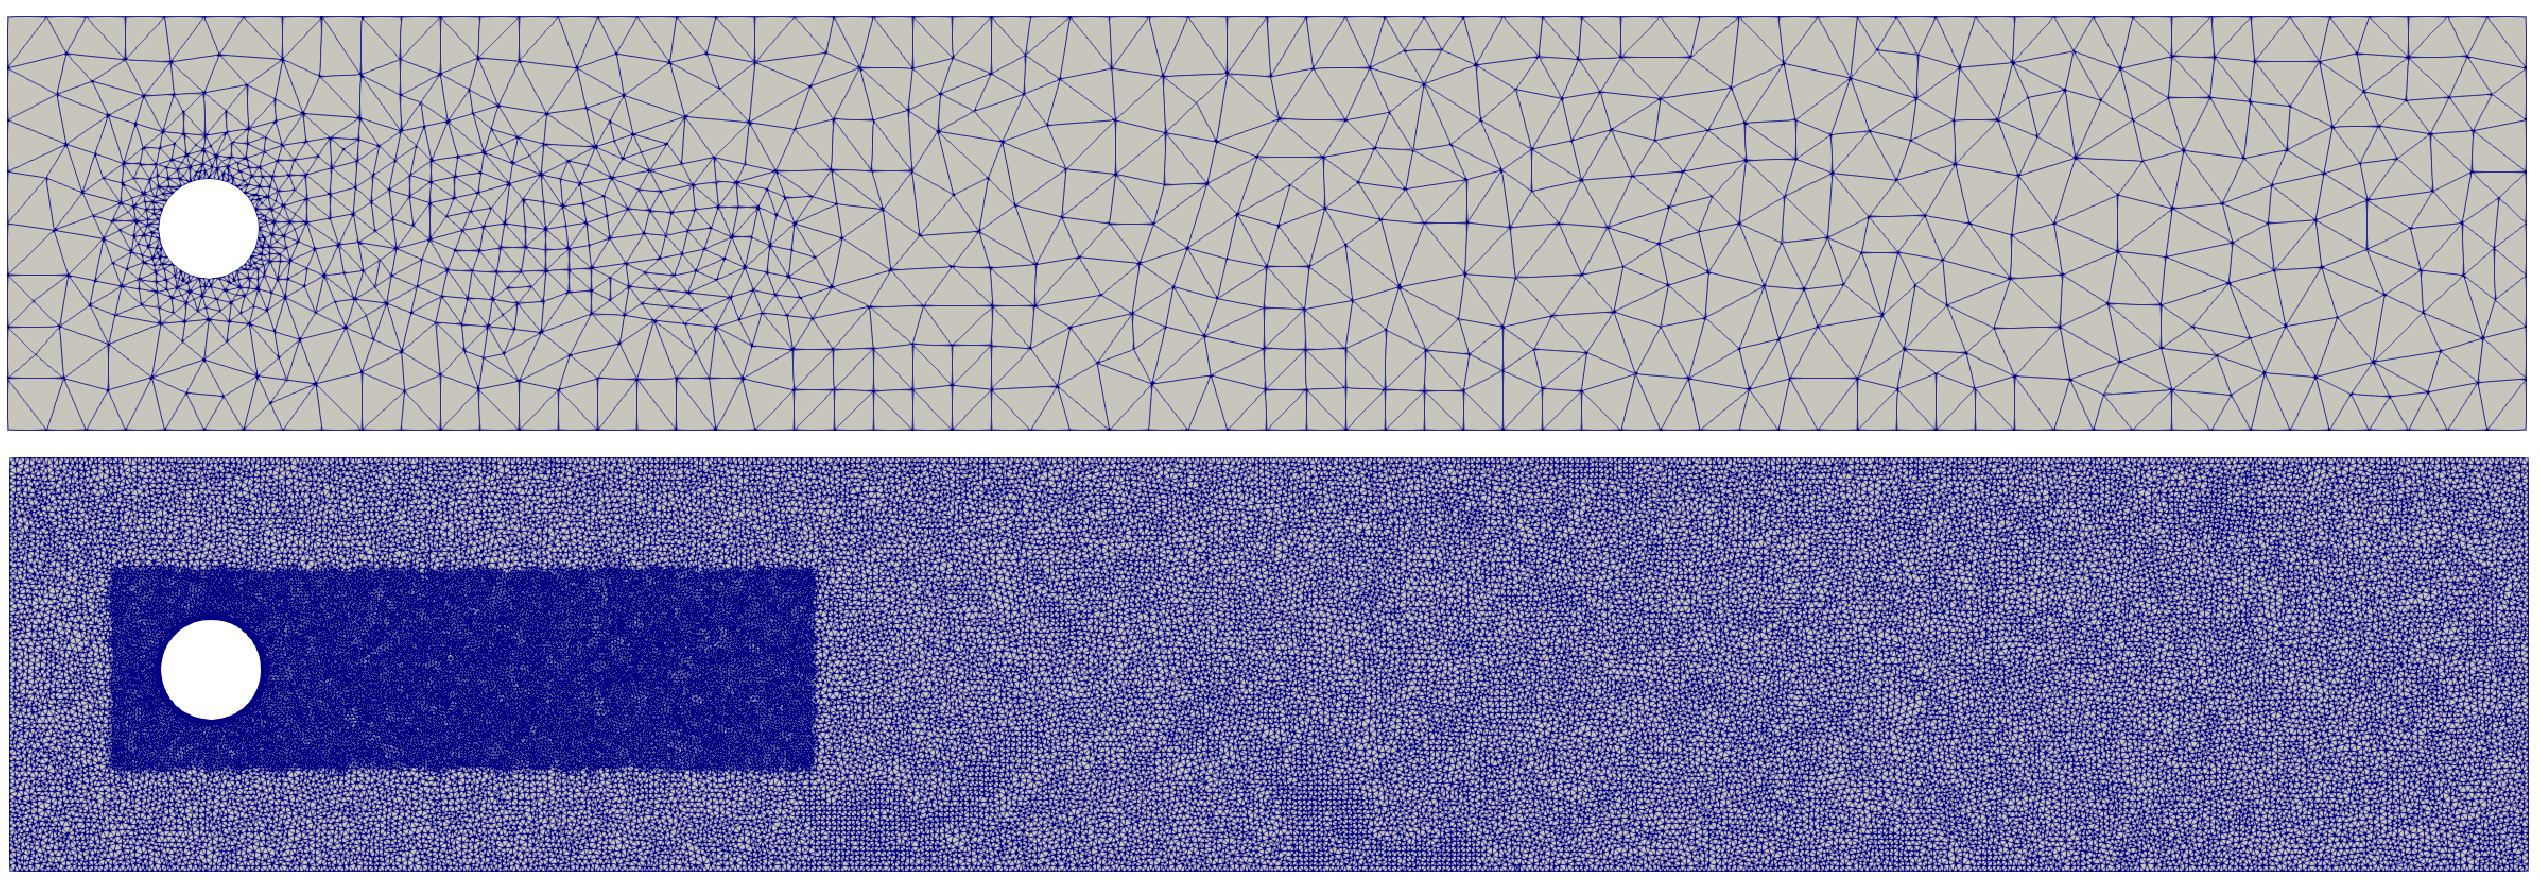
\includegraphics[width=0.6\textwidth]{mesh}
	\caption{Course mesh, $N = 32$ and most refined mesh, $N = 256$}
	\label{fig:mesh}
\end{figure}
\FloatBarrier

\section{Validation} 

The mesh refinement results of $C_D$, $C_L$ and $P_{diff}$ are presented in Table \ref{tab:fluid}. Figures \ref{fig:drag}, \ref{fig:lift} and \ref{fig:p_diff} illustrate mesh convergence to the benchmark solution for coefficients of drag and lift, and the pressure difference respectively. The red lines indicate the benchmark solution lower and upper bounds \cite{schafer1996benchmark}.   

\FloatBarrier
  \begin{table}[htbp]
  \setlength\extrarowheight{5pt}
  \centering
  \caption{Results of mesh independence study}
    \begin{tabular}{ccccc}
    \toprule
    $N$ & $ndof$ & $C_D$ & $C_L$ & $P_{diff}$ \\
    \midrule
$32$ & $8503$ & $5.512$ & $-0.01117$ & $0.1142$ \\
$64$ & $28760$ & $5.557$ & $0.01018$ & $0.1169$ \\
$128$ & $108217$ & $5.569$ & $0.01103$ & $0.1173$ \\
$256$ & $416630$ & $5.574$ & $0.01094$ & $0.1174$ \\
    \bottomrule
    \end{tabular}%
  \label{tab:fluid}%
\end{table}%
\FloatBarrier


\FloatBarrier
\begin{figure}[h]
\centering
	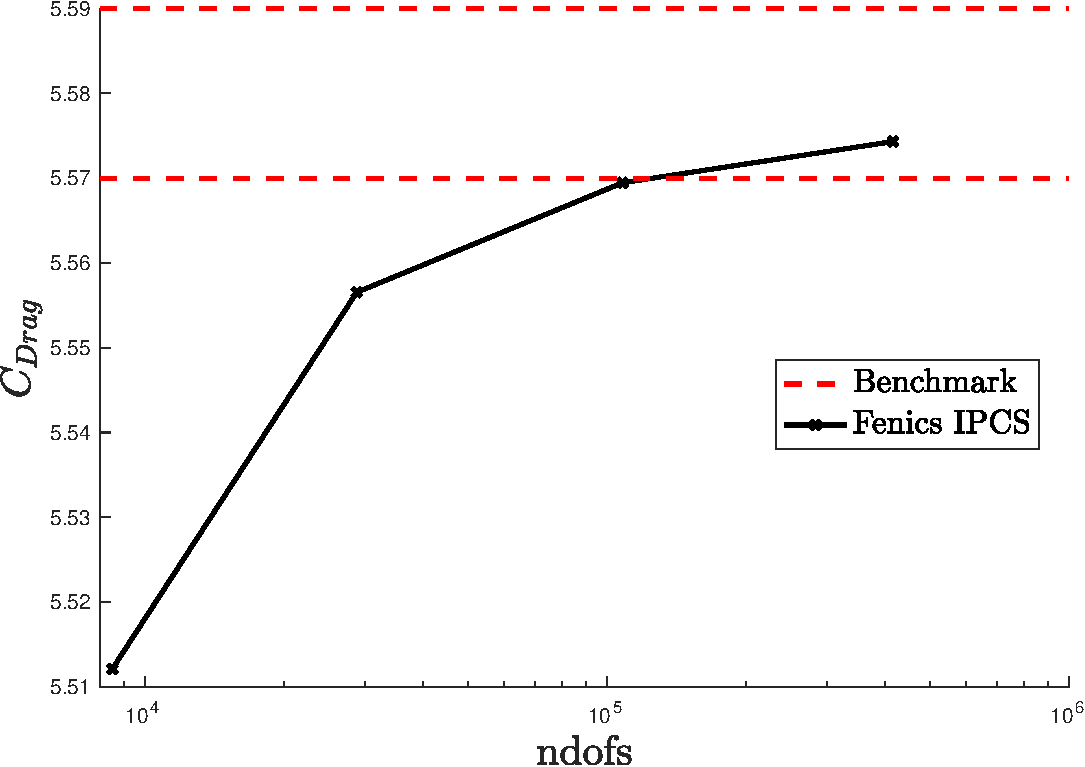
\includegraphics[width=0.6\textwidth]{drag-crop}
	\caption{Drag coefficient convergence to benchmark values}
	\label{fig:drag}
\end{figure}
\FloatBarrier


\FloatBarrier
\begin{figure}[h]
\centering
	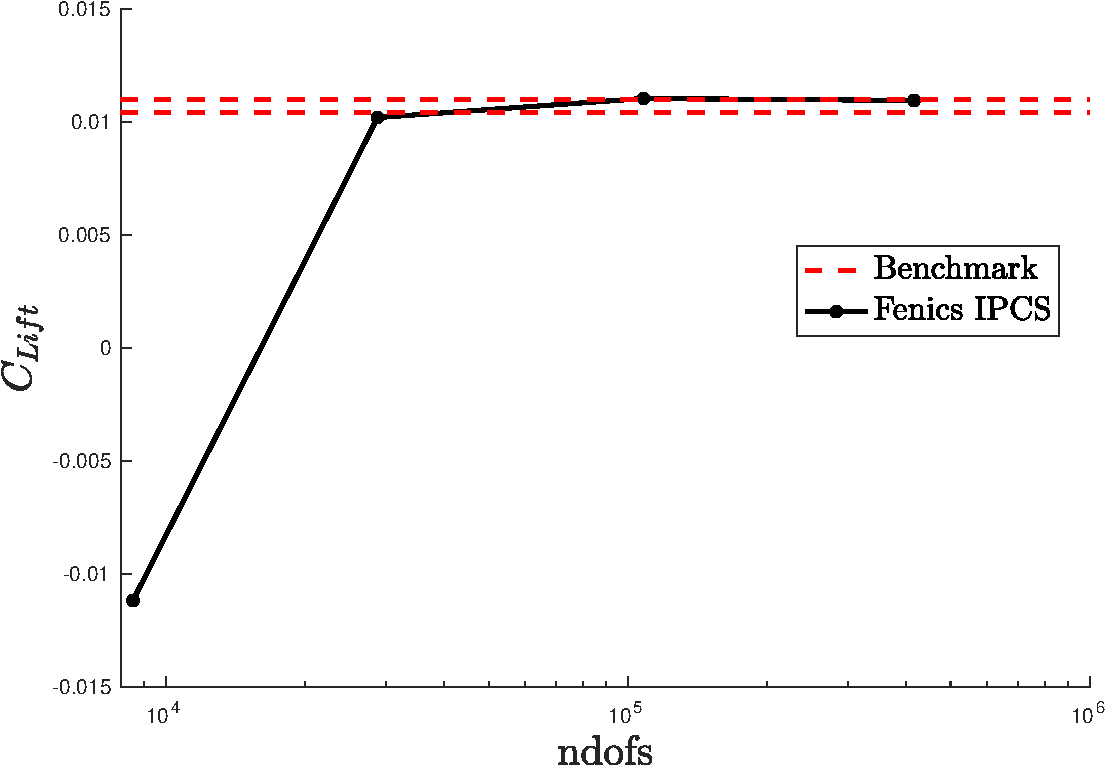
\includegraphics[width=0.6\textwidth]{lift-crop}
	\caption{Lift coefficient convergence to benchmark values}
	\label{fig:lift}
\end{figure}
\FloatBarrier



\FloatBarrier
\begin{figure}[h]
\centering
	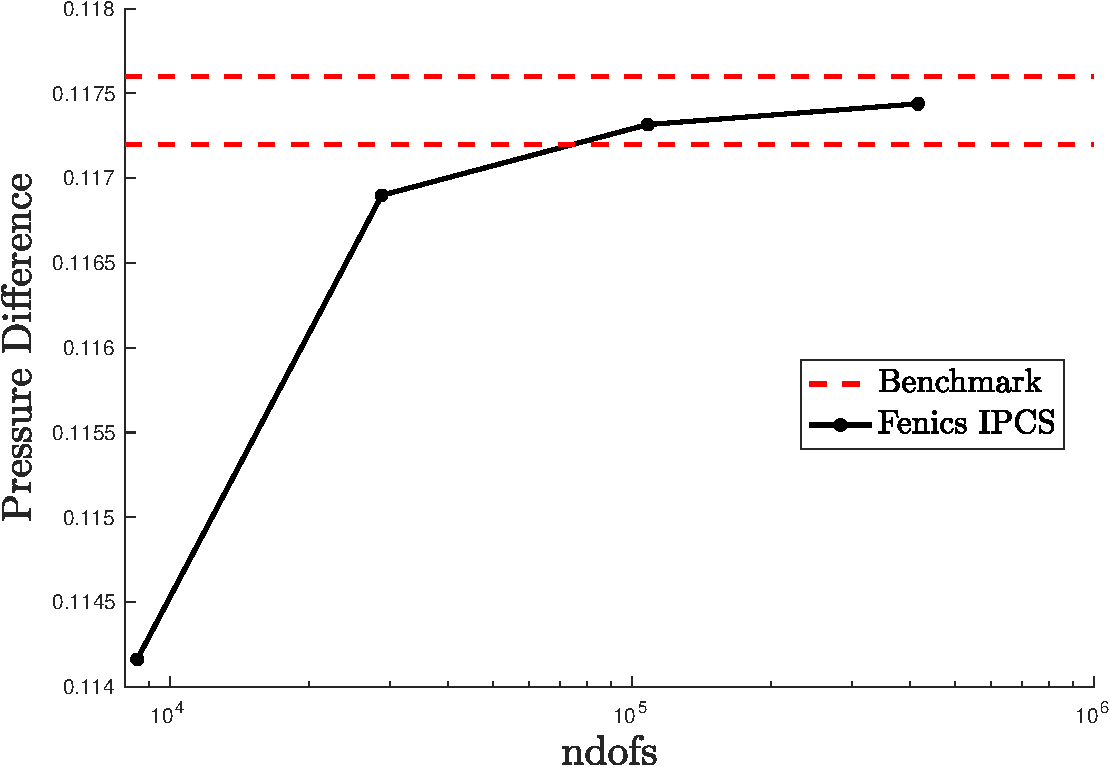
\includegraphics[width=0.6\textwidth]{p_diff-crop}
	\caption{Pressure difference convergence to benchmark values}
	\label{fig:p_diff}
\end{figure}
\FloatBarrier

Figures \ref{fig:drag}, \ref{fig:lift} and  \ref{fig:p_diff} all demonstrate convergence to the benchmark solution. Further mesh refinement is necessary to confirm mesh independence. The majority of the 17 methods presented in the benchmark solution to arrive at the bounds have a much higher grid refinement, 6 of them have an order of magnitude more more dofs. 

\section{FSI Application} 

I think these results are sufficient for application of this Fluid solver to a Fluid Structure Interaction problem. There remains some oscillatory behavior in the early development of the solution. Figure \ref{fig:dt_bench} depicts $C_L$ for the initial 50 time steps on the course mesh of $N = 32$. Evidently the magnitude of the oscillations is reduced as the simulation progresses. A smaller time step causes a smaller magnitude in the oscillation. 

This behavior could have important ramifications for fluid structure interaction, depending on the manner in which the oscillatory force on the structure interacts with the movement of the structure itself. If non-physical behavior does result, several solutions are available. The first is to use a smooth increase in velocity as the starting procedure. This is implemented for the non-steady solutions in the FSI benchmark \cite{turek2006proposal}. An alternative, though less elegant approach would be to run the fluid solver on its own for a set number of timesteps before introducing interaction. 

\FloatBarrier
\begin{figure}[h]
\centering
	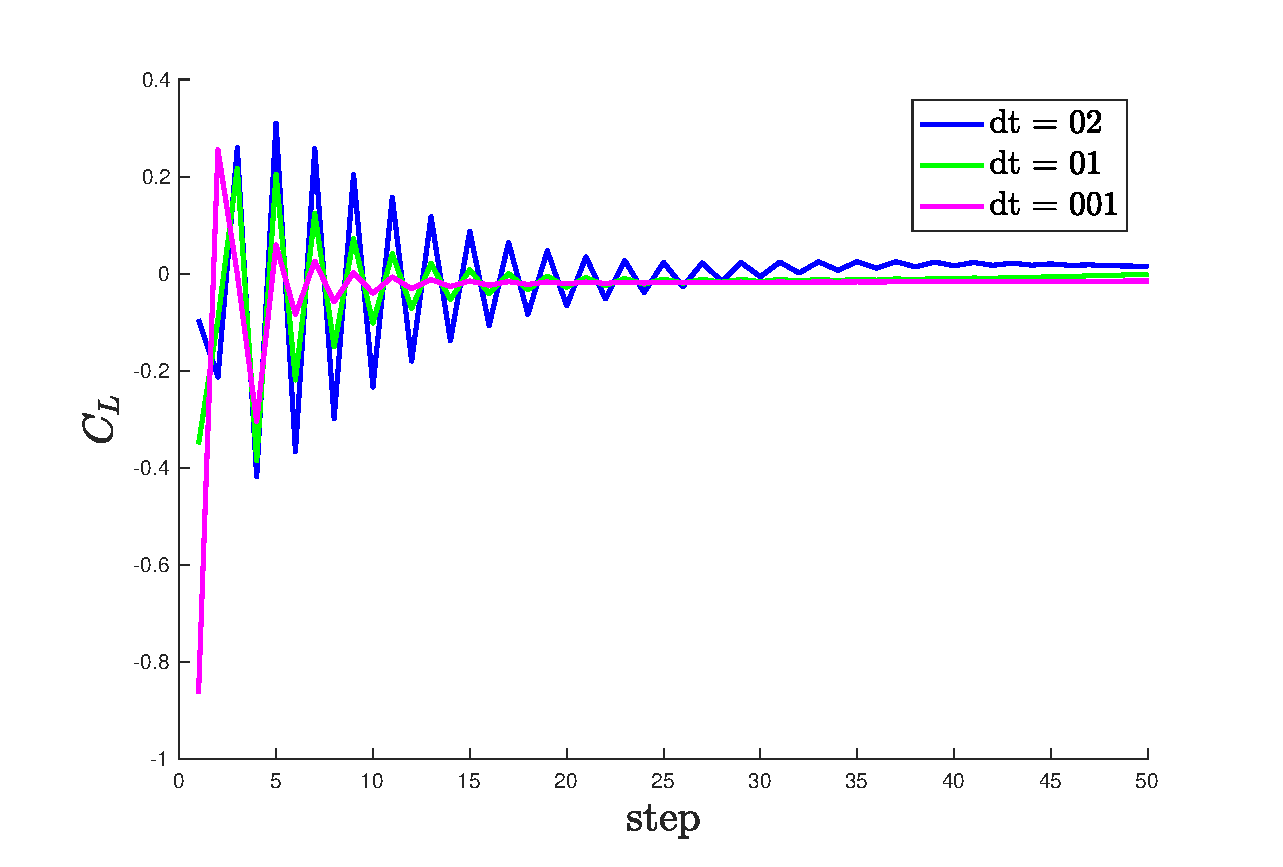
\includegraphics[width=0.6\textwidth]{dt_bench}
	\caption{Oscillatory behavior in $C_L$ with varying dt}
	\label{fig:dt_bench}
\end{figure}
\FloatBarrier

\bibliography{validation}{}
\bibliographystyle{plain}


\end{document}
